\documentclass{article}

\usepackage[T1]{fontenc}
\usepackage[utf8]{inputenc}
\usepackage[spanish]{babel}
\usepackage{graphicx}
\usepackage{microtype}
\usepackage{xcolor}
\usepackage{amsmath}
\usepackage{amssymb}
\usepackage{mathtools}
\usepackage{xfrac}
\usepackage{booktabs}
\usepackage{hyperref}
\usepackage{siunitx}

\newcommand{\todox}{\(\mathit{\color{red}x}\)}
\newcommand{\ham}{\large{\texttt{ham}}}
\newcommand{\spam}{\large{\texttt{spam}}}
\newcommand{\fo}{\(\mathbf{F_1}\)}

\interfootnotelinepenalty=10000

\title{Aprendizaje Automático \\ Trabajo Práctico 1 --- Detección de Spam}
\author{Martín Fixman \and Leandro Matayoshi \and Fernando Gasperi}
\date{Segundo Cuatrimestre de 2016}

\begin{document}
\maketitle

\newpage

\section{Introducción}

En este trabajo se midel diferentes basado en técnicas de \textbf{Apredizaje Automático} para clasificación de mails entre \ham{} o \spam{}.

La entrada consiste de \num{45000} mensajes clasificados a priori como \ham{}, y otros \num{45000} clasificados a priori como \spam{}. Para ayudar a medir las inferencias, tomamos el 10\% de cada uno de estos (\num{4500} \ham{} y \num{4500} \spam{}) como \textit{testing set}, y no hacemos ningún experimento sobre estos hasta el final del trabajo, cuando se miden los modelos.

\section{Extracción de Atributos}

\subsection{Análisis de texto}

Para obtener atributos relacionados con análisis de texto decidimos trabajar específicamente con 2 campos: \(body\) y \(subject\).

La extracción se realizó en base a aplicar Bayes sobre la probabilidad de que un mensaje sea \spam{} dada la aparición de una palabra (potencial atributo) en dicho mensaje.

Sea $w \in W$, siendo $W$ el universo de palabras obtenido a partir de los mails utilizados para entrenar el modelo.

\vspace{5px}
$P(spam \vert w) = \frac{P(w \vert spam) \cdot P(spam)}{P(w)}$, donde:

\vspace{5px}
$P(w \vert spam) = \frac{\sum_{s \in spam}^{} w \in s}{\mid spam \mid}$, $P(w) = \frac{\sum_{m \in M}^{} w \in m}{\mid M \mid}$, $P(spam) = \frac{\mid spam \mid}{\mid M \mid}$

\vspace{5px}
Análogamente, se realiza la misma operación para analizar las palabras que aparecen en los mails de \ham{}.

El primer experimento consistió en encontrar las 100 palabras que aparezcan en el body de los mails, y que maximicen el valor de Bayes tanto para \spam{} como
para \ham{}. Dicho de otra forma, encontramos las 100 palabras más spammeras y las 100 palabras más hammeras que aparezcan en el \(body\) de los mails.

Posteriormente realizamos un segundo experimento, repitiendo el proceso para las palabras del \(subject\) de los mails.

Durante esta etapa utilizamos la clase \(CountVectorizer\) del módulo \(feature \ extraction\) de \(sklearn\). \(CountVectorizer\) admite como parámetro un token-pattern,
que determina la estructura que deben seguir las palabras analizadas para ser consideradas potenciales features. En este caso, luego de probar con varios valores, optamos
por elegir palabras que contengan solo caracteres entre [a-z], y de longitud mínima = 4. Al mismo tiempo, también admite un parámetro que determina
la cantidad mínima de apariciones que debe tener una palabra para ser considerada \(token\). En este caso, luego de probar con varios valores, determinamos los valores de
800 apariciones para el caso del \(body\) y 200 para el \(subject\). Es decir, solo las palabras que aparecen como mínimo esa cantidad de veces entre la totalidad de
los mails fueron consideradas como tokens.


\section{Selección de Modelos}

En el punto anterior logramos conseguir una \textbf{Matriz de Features} \( X \), con \num{1068} columnas (features) y \num{81000} filas (samples), y un vector de clases \( y \) con \textbf{81000} samples, donde cada una indica si cada sample debería pertenecer a \ham{} o a \spam{}. Dadas estos datos, vamos a elegir varios modelos que pueden lograr seleccionar el modelo óptimo para la inferencia.

\subsection{Metodología de Puntaje}

El objetico de esta sección es mostrar varios métodos diferentes de predicción. Por esta razón, la comparación entre varios métodos se hace solo midiendo \textbf{accuracy}, o la cantidad de predicciones correctas del modelo. Más adelante se hace una comparación más contindente y con más parámetros.

Este trabajo separa métodos con 5 métodos diferentes para encontrar su precisión: \textbf{accuracy}, o la proporción de mails correctamente clasificados, \textbf{auc}, el área bajo la curva ROC de una corrida del método, \textbf{precision} y \textbf{recall}, que miden cuán buena es la predicción para instancias positivas\footnote{En el caso de este trabajo, se toma ``instancia positiva'' como un mensaje de \textbf{spam}; de esta manera un \textbf{True Positive} es un mensaje de spam bien clasificado mientras que un \textbf{False Negative} es un mensaje de spam clasificado como ham}, y el \fo-score, que analiza estos dos valores de igual manera.

Como parte del trabajo es analizar la \textit{performance} de los clasificadores, se agregan dos nuevas medidas: \textbf{fit\_time}, el tiempo que tarda el hacer \textit{fitting} a los casos de entrenamiento, y \textbf{predict\_time}, el tiempo que tarda en hacer las predicciones de los casos de test.

Para prevenir los casos de overfitting, se usa \textbf{Stratified K-Folds} validation como validación cruzada, eligiendo un valor de \( k = 10 \)\footnote{Este valor nos pareció un poco elevado para este caso, pero este es el más comunmente usado}. De esta manera, tomamos el accuracy, auc, precision, recall, y \(F_1\)-score como el promedio de estos valores; esto es una agregación estadísticamente buena\cite{forman2010}.

Adicionalmente, todos los modelos que requieran algo de azar se ejecutan con la misma raíz (\texttt{random\_state es 0}); de esta manera se puede facilmente replicar los experimentos.

\subsection{Decision Tree}

La manera más simple de decidir a qué categorías pertenecen los mails con features similares a los de \( X \) es usar un árbol de decisión.

Además de ser muy sensible al overfitting, la versión ``regular'' de este método que usa todos los features e intenta crear un árbol lo más grande posible es demasiado lenta para nuestro caso, por lo tanto elegimos limitar la cantidad máxima de features y la altura del árbol a la raíz cuadrada de la cantidad de features (\(\lceil\sqrt{1068}\rceil = 33\)), y a la altura máxima de 10. Estos valores fueron elegidos entre otros ya que dan un buen resultado, mientras que también terminan en un tiempo razonable y terminan en árboles lo suficientemente chicos para que el overfitting no sea una gran preocupación.

Luego de aplicar \textbf{Stratified 10-Folds}, llegamos a un score promedio de \( \mathbf{0.982} \).

\begin{figure}
	\centerline{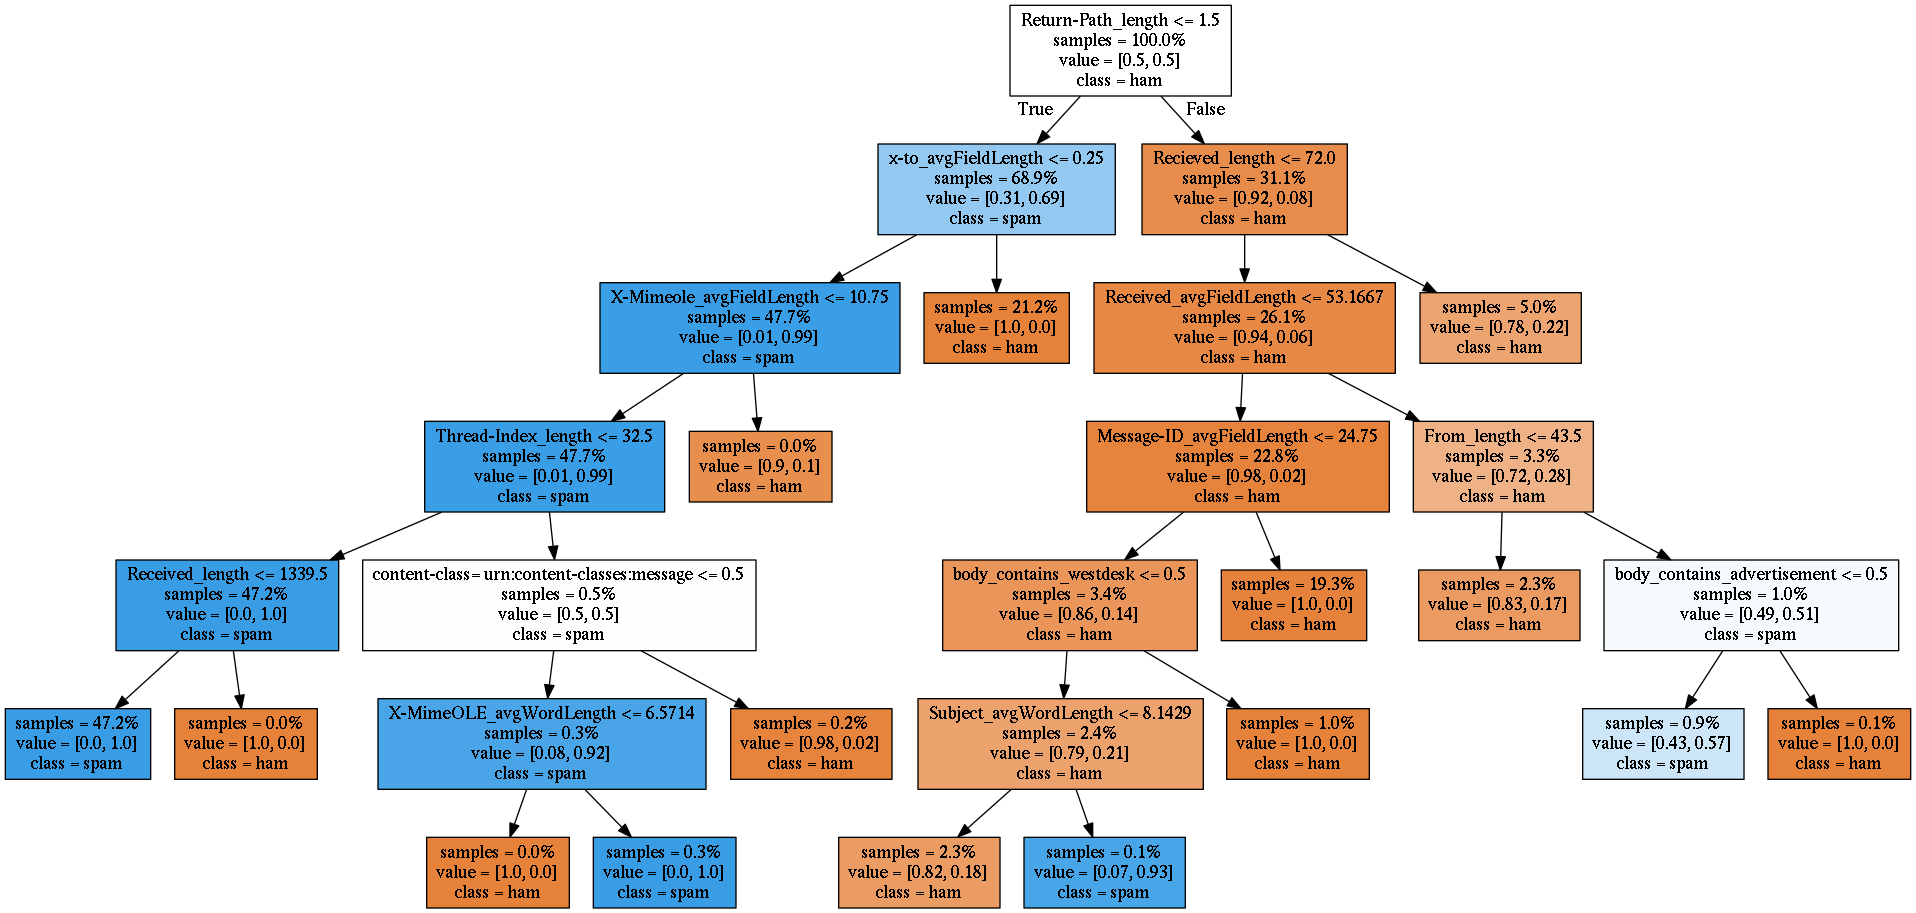
\includegraphics[width=1.3\textwidth]{tree.png}}
	\caption{Árbol de decisión similar con un score un poco menor (pero que es mucho más lindo a la vista).}
\end{figure}

\subsection{Naive Bayes}

Se prueba usar el modelo de Bernoulli usado en sklearn en las variables booleanas del modelo. El único hiperparámetro para elegir es \( \alpha \), el nivel de ``smoothing'' and se le hace a la entrada.

Adicionalmente, los features se separaron en 5 subconjuntos:
\begin{itemize}
	\item \textbf{Existente} Los features \texttt{*\_exists}, que dicen si un campo del header existe o no.
	\item \textbf{Header features} Los features que dan información sobre estos campos.
	\item \textbf{Categorization} Los features que dicen qué valores toman algunos campos.
	\item \textbf{Word bag} Que dicen si cada palabra apareció o no en el mail.
	\item \textbf{Binary} Todos los features binarios, eso es \( \text{Existente} \cup \text{Word Bag} \).
\end{itemize}

Se corrió el estimador de Naive Bayes usando estos subconjuntos de features y diferentes \( \alpha \) y se midió el accuracy de los resultados.

\begin{figure}
	\centerline{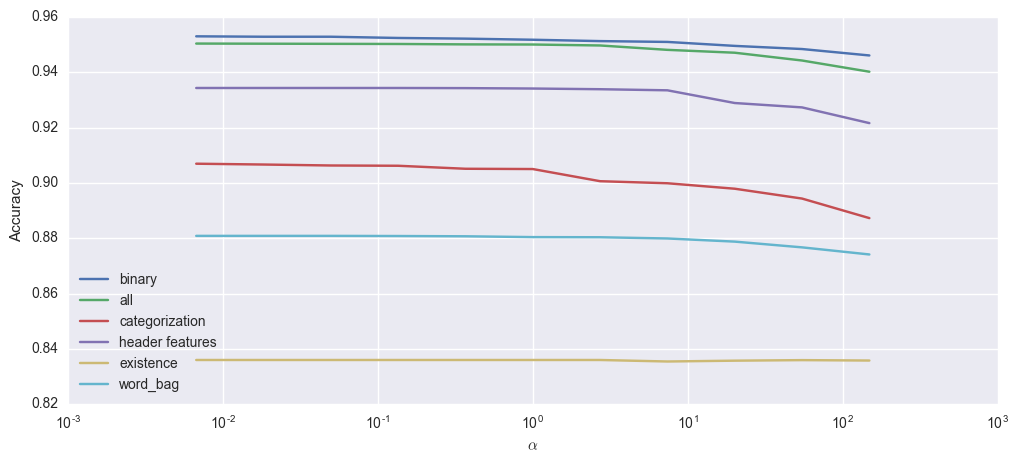
\includegraphics[width=1.3\textwidth]{figures/bayes.png}}
	\caption{Accuracy de los experimentos}
\end{figure}

Se puede ver que el categorizador que usa features binarios suele ser el mejor, y que el accuracy sube cuando baja el smoothing (aunque cuando \( \alpha = 0 \) el accuracy se vuelve particularmente malo). Como de cualquier manera la diferencia es mínima, tomamos \( \alpha = 1 \) y usamos todos los features.

\subsection{K Nearest Neighbors}

Otro estimador que se usó para intentar inferir si un mail es spam o no es el de \textbf{K nearest neighbors}, que decide si un punto forma parte de cada categoría dependiendo de la cantidad o la distancia de puntos de cada categoríá entre los \( K \) que estén a menor distancia Euclideana (u otra medida de distancia).

Dado que hay una gran cantidad de posibles combinaciones para \( K \), y que no se sabe si el mejor estimador usa mayoría absoluta o la suma de las distnacias, se hizo un \textbf{Grid Search} para buscar el valor óptimo de estos parámetros.

\begin{center}
\begin{tabular}{c c c c}
	\toprule
	\textbf{Pesos} & \textbf{K} & \textbf{Avg.\ score} & \textbf{Std.\ score} \\
	\midrule
	uniform & 3 & 0.91765 & 0.00451 \\
	uniform & 5 & 0.90988 & 0.00276 \\
	uniform & 7 & 0.90815 & 0.00134 \\
	distance & 3 & 0.92062 & 0.00408 \\
	distance & 5 & 0.91778 & 0.00214 \\
	distance & 7 & 0.91679 & 0.00048 \\
	\bottomrule
\end{tabular}
\end{center}

Se puede ver que, antiintuitivamente, el méþodo da mejor cuando se toman menos vecinos pero se mide por distancia.

También se intentó hacer una normalización normal a los features, que centra cada componente a uno que tenga media \( \mu = 0 \) y varianza \( \sigma^2 = 0 \).

\[
	f' = \frac{f - \mu_f}{\sigma_f} \; (\forall f \in \text{Features})
\]

De esta manera se le puede dar aproximadamente el mismo peso a cada uno de los features en los métodos. Esto se puede ver en la diferencia con el método anterior.

\begin{center}
\begin{tabular}{c c c c}
	\toprule
	\textbf{Pesos} & \textbf{K} & \textbf{Avg.\ score} & \textbf{Std.\ score} \\
	\midrule
	uniform & 3 & 0.97531 & 0.00107 \\
	uniform & 5 & 0.97296 & 0.00229 \\
	uniform & 7 & 0.97420 & 0.00185 \\
	distance & 3 & 0.97716 & 0.00123 \\
	distance & 5 & 0.97765 & 0.00140 \\
	distance & 7 & 0.97852 & 0.00229 \\
	\bottomrule
\end{tabular}
\end{center}

Los resultados son considerablemente mejores que la versión sin normalización, por lo que vale la pena normalizar los datos. Además, se puede ver que esta vez sí mejora la accuracy cuando aumenta la cantidad de vecinos; de cualquier manera el aumento es mínimo, y conviene seguir usando 3 vecinos (y medir los pesos por distancia) ya que el método es mucho más rapido.

\subsection{Nearest Centroid}

Esta es una alternative a \textbf{K Nearest Neighbors} donde cada clase se representa por una solo centroide. Aunque parecía tentadora debido a la nula cantidad de parámetros posibles, este método dio un accuracy promedio abismal de \( 0.471 \). Por esta razón no se incluye en el resto de los análisis.

\subsection{Support Vector Machines}

Se usaron \textbf{Support Vector Machines}, que intentan buscar el hiperplano que mejor separa el espacio en dos conjuntos lo más diferentes posibles. Debido a la funcionalidad de este clasificador, se noemalizaron los features de la misma maenra que en la sección de \textbf{K Nearest Neighbors}.

Los tres parámetros importantes de SVM lineal (cuando no se usa el truco de los kernels) son \textbf{C}, que mide la penalidad de un error, \textbf{penalty} decide qué norma usar para medirlo, y \textbf{loss}, que elige una función para normalizar. En los casos donde se usa squared hinge elegimos usar optimización primal contra dual, ya que tenemos una cantidad de samples mucho mayor a la cantidad de features\cite{ngcs229}.

\begin{center}
\begin{tabular}{r c l c c}
	\toprule
	\textbf{C} & \textbf{Penalty} & \textbf{Loss} & \textbf{Avg.\ score} & \textbf{Std.\ score} \\
	\midrule
	0.01 & l1 & squared hinge & 0.97864 & 0.00310 \\
	0.01 & l2 & squared hinge & 0.98519 & 0.00052 \\
	0.01 & l2 & hinge & 0.98506 & 0.00227 \\
	0.1 & l1 & squared hinge & 0.98556 & 0.00181 \\
	0.1 & l2 & squared hinge & 0.98284 & 0.00114 \\
	0.1 & l2 & hinge & 0.98284 & 0.00106 \\
	1 & l1 & squared hinge & 0.98296 & 0.00160 \\
	1 & l2 & squared hinge & 0.98136 & 0.00114 \\
	1 & l2 & hinge & 0.97840 & 0.00251 \\
	10 & l1 & squared hinge & 0.98259 & 0.00297 \\
	10 & l2 & squared hinge & 0.98198 & 0.00149 \\
	10 & l2 & hinge & 0.97901 & 0.00274 \\
	100 & l1 & squared hinge & 0.98296 & 0.00181 \\
	100 & l2 & squared hinge & 0.98160 & 0.00155 \\
	100 & l2 & hinge & 0.97901 & 0.00274 \\
	\bottomrule
\end{tabular}
\end{center}

Se puede ver que los mejores puntajes se dieron cuando se minimiza \textbf{C}, y que la función cuadrática de pérdida (squared hinge) es un poco mejor que la cuadrada que se usa en los kernels lineales. Además, cuando se usa esta función, usar la norma \(l2\) suele dar un mejor resultado que con la norma \(l1\).

\subsubsection{Kernel Trick}

\textbf{Support Vector Machines} tiene la posibilidad de usar el \textbf{kernel trick}, que aplica funcionar a conjuntos de features para conseguir nuevos features y ``simular'' una función de separación que sea más compleja que un hiperplano.

Como el algoritmo regular para entrenar SVM tarda un tiempo cuadrático en la cantidad de samples, es demasiado lento para hacer grid search con una cantidad significativa de folds para medir hiperparámetros. Por esa razón, usamos un sample de \(\sfrac{1}{10}\) de los mails a la hora de elegir los mejores hiperparámetros para los estimadores.

Se hizo un \textbf{Grid Search} con tres diferentes kernels en SVM para elegir hiperparámetros.

\begin{itemize}
	\item \textbf{\(\mathbb{P}^2\)} Polinomio de grado 2.
	\item \textbf{\(\mathbb{P}^3\)} Polinomio de grado 3.
	\item \textbf{RBF} Kernel Gaussiano que intenta hacer un circulo.
\end{itemize}

\begin{center}
\begin{tabular}{r r c c}
	\toprule
	\textbf{Kernel} & \textbf{C} & \textbf{Avg.\ score} & \textbf{Std.\ score} \\
	\midrule
	\(\mathbb{P}^2\) & 0.001 & 0.50222 & 0.00000 \\
	\(\mathbb{P}^3\) & 0.001 & 0.50222 & 0.00000 \\
	\(\mathbb{P}^2\) & 0.01 & 0.57975 & 0.01614 \\
	\(\mathbb{P}^3\) & 0.01 & 0.55037 & 0.00939 \\
	RBF & 0.01 & 0.87605 & 0.00817 \\
	\(\mathbb{P}^2\) & 0.1 & 0.94000 & 0.00682 \\
	\(\mathbb{P}^3\) & 0.1 & 0.88370 & 0.01782 \\
	RBF & 0.1 & 0.92864 & 0.01347 \\
	\(\mathbb{P}^2\) & 1 & 0.95679 & 0.00635 \\
	\(\mathbb{P}^3\) & 1 & 0.94691 & 0.00609 \\
	RBF & 1 & 0.97531 & 0.00344 \\
	\(\mathbb{P}^2\) & 10 & 0.98420 & 0.00194 \\
	\(\mathbb{P}^3\) & 10 & 0.96247 & 0.00286 \\
	RBF & 10 & 0.98222 & 0.00060 \\
	\(\mathbb{P}^2\) & 100 & 0.98370 & 0.00264 \\
	\(\mathbb{P}^3\) & 100 & 0.98420 & 0.00140 \\
	RBF & 100 & 0.98272 & 0.00252 \\
	\(\mathbb{P}^2\) & 1000 & 0.98222 & 0.00277 \\
	\(\mathbb{P}^3\) & 1000 & 0.98222 & 0.00277 \\
	RBF & 1000 & 0.98222 & 0.00277 \\
	\bottomrule
\end{tabular}
\end{center}

Se puede ver que el kernel cúbico, \(\mathbb{P}^3\) es el que da el mejor resultado, y que esto mejora cuando \( C = 100\). Sin embargo, el accuracy de este método sigue siendo peor al de SVM sin usar un kernel, además de ser bastante más lento.

\subsection{Random Forest}

Un método de ensamble bastante simple es \textbf{Random Forest}, que tiene una buena accuracy como un Decision Tree pero es mucho menos probable caer en overfitting. Hay 3 posibles hiperparámteros que pueden afectar la velocidad y la accuracy con la que se hace la inferencia: la \textbf{cantidad} de árboles con los que se hace la estimación, la \textbf{profundidad} de los árboles, y la \textbf{cantidad de features} con los que se arma cada árbol.

Se puede ver trivialmente que cuanto más profundo sea cada árbol de un bosque y cuanta mayor cantidad de features haya mejor va a ser la predicción, aunque esta puede ser mucho más lenta y puede tener mayor probabilida de tener overfitting. Por eso, es necesario hacer un mejor análisis de los hiperparámetros.

\begin{figure}
	\centerline{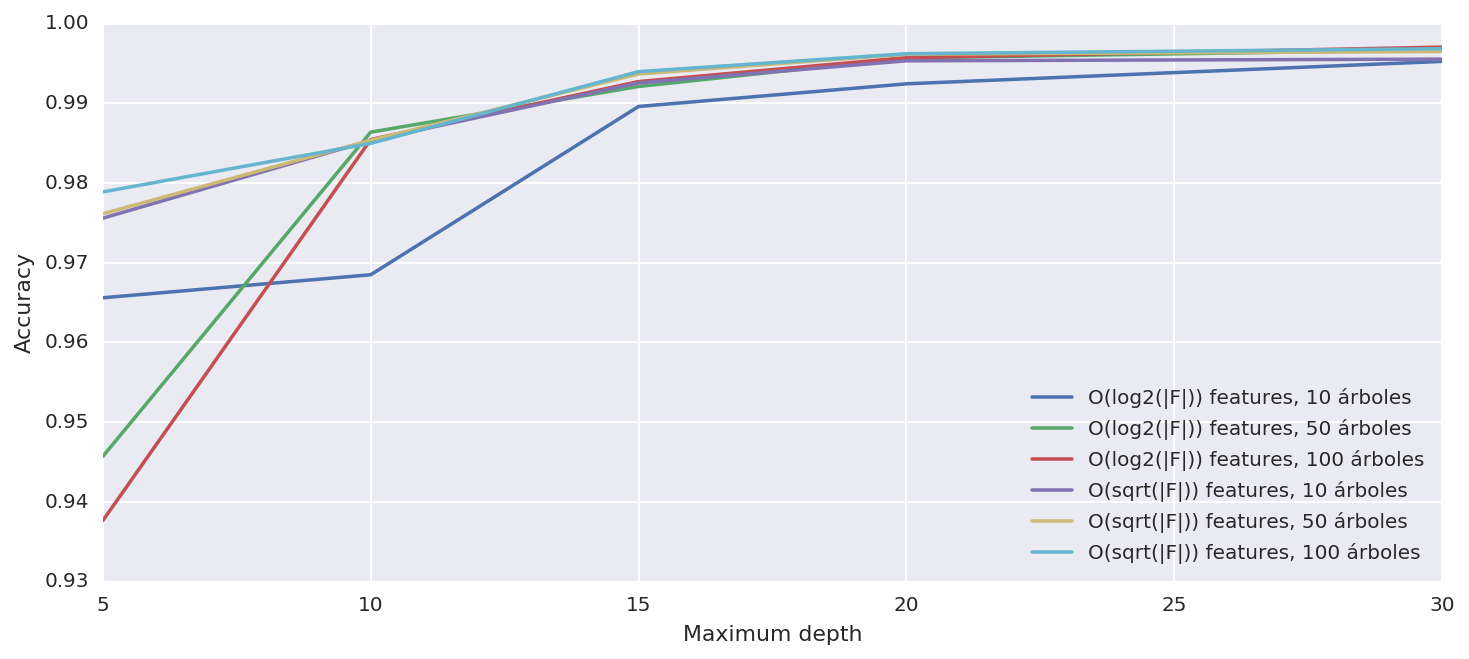
\includegraphics[width=1.3\textwidth]{figures/forest.png}}
	\caption{Accuracy de diferentes Random Forests, testeado con K-folds}
\end{figure}

Se puede ver que usar una cantidad cercana a \( \sqrt{\left|F\right|} \) (donde \(\left|F\right|\) es la cantidad de features) de los features es más conveniente, Por otro lado, y antiintuitivamente, la cantidad de árboles no mejora el puntaje, aunque hace mucho más lenta la predicción!

Basado en estos datos, elegimos usar \( \sqrt{|F|} \) features, 10 árboles, y una profundidad máxima de 15 nodos.

\subsection{Voting}

Una manera simple de combinar varios estimadores en un ensemble es haciendo un ensemble y una votación entre ellos.

\subsubsection{Absolutamente todo}

La manera más obvia de usar este método es usar una votación entre los 5 métodos con mejor accuracy:

\begin{itemize}
	\item Un árbol de decisión con a lo sumo \( \sqrt{\left|F\right|} \) features, 15 nodos hoja y máxima profundidad de 7 nodos.
	\item Naive Baytes, con \( \alpha = 1 \).
	\item K Nearest Neighbors, con 7 vecinos medidos por distnacia.
	\item Support Vector Machines, sin usar kernels, con \( C = 0.01 \), y midiendo por norma l2.
	\item Random Forest, con \( \sqrt{\left|F\right|} \) features, 10 árboles, y a lo sumo 15 nodos hoja.
\end{itemize}

Midiendo el voto mayoritario usando K-folds, conseguimos un accuracy de \( 0.983 \).

\subsubsection{Voto calificado}

Otra posible técnica es hacer esto mismo, pero en vez de elegir el voto mayoritario, darle un puntaje a cada estimador dependiendo de cuan bien de la inferencia. Desafortunatemente, esto parece darle ventaja a los estimadores malos: el accuracy promedio de los folds es de \( 0.956 \).

\subsubsection{Ensambles con menos estimadores}

Se consiguió una buena estimación haciendo votación con una menor cantidad de estimadores. En particular, juntando \textbf{Random Forest}, \textbf{K nearest neighbors}, y \textbf{Support Vector Machines} sin kernels, se llegó a un accuracy de \( 0.986 \).

\section{Reducción de Dimensionalidad}

\subsection{Experimentación inicial}

Como primera aproximación para reducir la cantidad de atributos utilizamos los algoritmos \textbf{SelectKBest} y \textbf{SelectPercentile} de
la sklearn.feature\_selection. La función de \( score \) elegida para ambos algoritmos fue \( chi2 \), y los features utilizados para la
experimentación fueron los Word Bags, tanto del body como del subject de los mensajes.

Luego de aplicar los algoritmos de reducción, utilizamos el modelo Bernoulli (Naive Bayes) como estimador para obtener el \( accuracy \) resultante
de la transformación de los datos.

\textbf{SelectKBest} toma un parámetro \( k \) que determina la cantidad de atributos a los cuales ajustarse.
\textbf{SelectPercentile} toma un parámetro \( p \) que determina un porcentaje de atributos a los cuales ajustarse.

A continuación se muestran los resultados obtenidos:

\begin{figure}
	\centerline{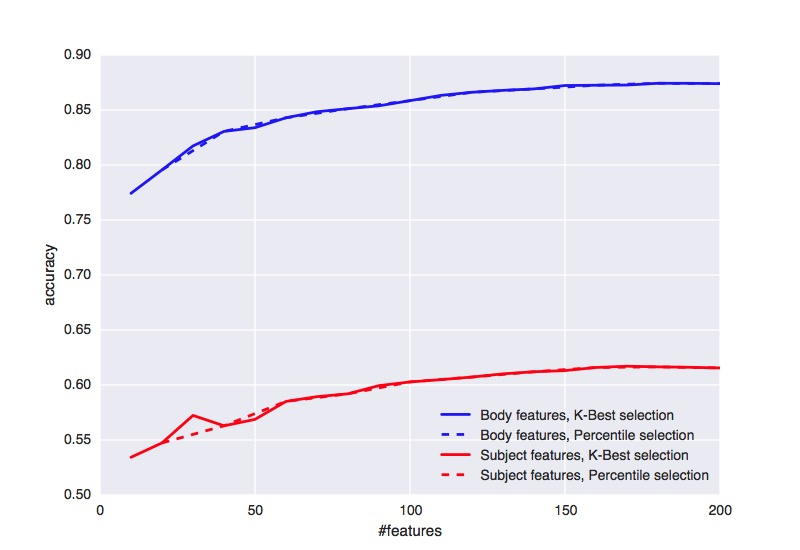
\includegraphics[scale=0.4]{figures/bernoulli_reduced_dimensionality.jpg}}
	\caption{Accuracy en función de cantidad de features resultante}
\end{figure}

La observación inmediata es que ninguno de los 2 algoritmos logra incrementar el accuracy al reducir la cantidad de atributos. De hecho, el accuracy máximo
se alcanza cuando el estimador utiliza la totalidad de los features. Es decir, no se produce reducción alguna.

Una segunda observación es que ambos algoritmos tienen una performance muy similar, si bien KBest parece dar un mejor resultado con una cantidad
de features menor.


\section{Resultados}

Se miden los estimadores usando el test set del 10\% de los mails, que no se tocó hasta este momento.

\renewcommand{\thefootnote}{\fnsymbol{footnote}}

\centerline{\begin{tabular}{r c c c c c c}
	\toprule
	\textbf{estimator} & \textbf{accuracy} & \textbf{auc} & \textbf{precision} & \textbf{recall} & \textbf{\(F_1\)-score} & \textbf{Predict time (s)} \\
	\midrule
	kNN & 0.967 & 0.984 & 0.965 & 0.97 & 0.967 & 117.0 \\
	LinearSVC & 0.971 & \footnotemark[1] & 0.971 & 0.971 & 0.971 & 0.218 \\
	NaiveBayes & 0.911 & 0.969 & 0.861 & 0.98 & 0.916 & 1.218 \\
	RandomForest & 0.960 & 0.994 & 0.990 & 0.929 & 0.959 & 0.033 \\
	VotingAll & 0.973 & \footnotemark[1]  & 0.991 & 0.955 & 0.973 & 125.6 \\
	VotingFew & 0.976 & \footnotemark[1] & 0.984 & 0.968 & 0.976 & 125.5 \\
	SoftVoting & 0.968 & \footnotemark[1] & 0.971 & 0.963 & 0.967 & 203.8 \\
	\bottomrule
\end{tabular}}

Podemos ver que, entre los métodos simples, el de \textbf{Support Vector Machines} tiene el mejor resultado, y hasta hacer la predicción es mucho más rápido que con otros métodos. Por otro lado, el método \textbf{VotingFew}, que usaba una combinación de Random Forest, K nearest neighbrs, y Support Vector Machines tiene un mejor accuracy y mejor de todos los otros puntajes que se pueden calcular, aunque es mucho más lento que el anterior.

\subsection{Usando Principal Component Analysis}

Se hace el mismo estudio con los componentes resultantas de PCA

\centerline{\begin{tabular}{r c c c c c c}
	\toprule
	\textbf{estimator} & \textbf{accuracy} & \textbf{auc} & \textbf{precision} & \textbf{recall} & \textbf{f1-score} & \textbf{predict-times} \\
	\midrule
	DecisionTree-PC.p & 0.542 & 0.536 & 0.655 & 0.177 & 0.279 & 0.001 \\
	knn-PC.p & 0.702 & 0.728 & 0.707 & 0.689 & 0.698 & 6.364 \\
	linearSVC-PC.p & 0.671 & \footnotemark[1] & 0.709 & 0.580 & 0.638 & 0.075 \\
	NaiveBayes-PC.p & 0.499 & 0.649 & 0.482 & 0.003 & 0.006 & 0.177 \\
	randomforest-PC.p & 0.539 & 0.623 & 0.765 & 0.112 & 0.196 & 0.204 \\
	VotingAll-PC.p & 0.496 & \footnotemark[1] & 0.293 & 0.004 & 0.009 & 7.082 \\
	VotingFew-PC.p & 0.654 & \footnotemark[1] & 0.724 & 0.498 & 0.591 & 6.899 \\
	SoftVoting-PC.p & 0.596 & 0.753 & 0.729 & 0.306 & 0.431 & 10.383 \\
	\textbf{estimator} & \textbf{accuracy} & \textbf{auc} & \textbf{precision} & \textbf{recall} & \textbf{\(F_1\)-score} & \textbf{Predict time (s)} \\
\end{tabular}}

Se puede ver que, a diferencia de lo que dice la teoría, este modelo dió considerablemente peor que el modelo sin la transformación. Aunque es posible que esto sea algo que pase en este dataset, no descartamos que haya habido un error en la transformación de los datos de prueba y del score.

\footnotetext[1]{El modelo de SVC lineal usado para la predicción no permite conseguir la probabilidad de cada una de las predicciones, por lo que no se puede armar una curva ROC ni conseguir el área bajo esta.}
\section{Discusión}

Entre las principales conclusiones, destacamos:
\begin{itemize}
	\item La bibilioteca Sklearn de Python provee una documentación extensa y muy completa para atacar este tipo de problemas, lo que nos permitió experimentar con una gran variedad de algoritmos tanto de clasificación como de reducción de dimensionalidad
	\item Resulta muy útil separar un conjunto de datos de tests, además de entrenamiento
	\item Los componentes principales del training set son muy diferentes a los del testing set, posiblemente por la manera que se extraen los features
	\item Otros algoritmos de reducción no siempre mejoran la performance de los modelos
\end{itemize}

\section{Bibliografía}

\begin{thebibliography}{9}

\bibitem{forman2010}
	George Forman \\
	Apples-to-Apples in Cross-Validation Studies: Pitfalls in Classifier Performance Measurement \\
	Hewlett Packard Labs \\
	DOI 10.1.1.186.8880

\bibitem{ngcs229}
    Andrew Ng \\
	CS229 Lecture Notes \\
	\url{http://cs229.stanford.edu/notes/cs229-notes3.pdf}

\end{thebibliography}

\end{document}
